\documentclass[a4]{article}
\usepackage{graphicx}
\usepackage{algorithm}
\usepackage{algorithmic}
\usepackage{lscape}
\usepackage{hyperref}
\usepackage{amssymb,longtable}
\usepackage[centertags]{amsmath}
\usepackage{amsfonts}
\usepackage{amsthm}
\usepackage{newlfont}
\usepackage{caption}
\usepackage{epsfig}
\newcommand{\norm}[1]{\left\Vert#1\right\Vert}

\textwidth  17.17cm
\textheight 23.4cm
\oddsidemargin -0.7mm
\evensidemargin -0.7mm
\def\baselinestretch{1.1}

\topmargin -8.4mm

\begin{document}

\title{Software Outlook: FFT Benchmarks for Fortran Codes }
\author{H. Sue Thorne}

\maketitle

%\begin{abstract}
%The abstract text goes here.
%\end{abstract}

\section{Introduction}
As part of the 2018/19 Software Outlook Work Plan, we will be benchmarking 
a number of different Fast Four Transform (FFT) libraries with bindings for
Fortran. The attributes of the different libraries are given in 
Section~\ref{Sec:libs}. Assuming indexing starts at 1, the discrete 1D Fourier transform of a vector $x$ of length $n$ is defined as
\begin{equation}\label{Eqn:fft}
  z(k) = \sum_{m=1}^{n} x(m) \exp(-2\pi i (k-1) (m-1) / n), \quad l=1,\ldots,n.
\end{equation}
In this work, we consider FFT libraries that have both multi-threading (OpenMP) and MPI capabilities.

\subsection{Half-complex format}
For input data that is purely real, the discrete Fourier transform satisfies 
the ``Hermitian'' redundancy: in 1D, if $x$ is a real array, then $z$ computed 
via (\ref{Eqn:fft}) will be a complex array satisfying
$$z(k) = \left[z(n-k+2)\right]^*, \quad k=2,\ldots,n.$$ Also note that the 
imaginary part of $z(1)$ is always 0; for $n$ even, the imaginary part of 
$z(n/2 + 1) $ is also always 0. This special symmetry in $z$ is known as 
\textit{half-complex} format and means that it can 
be stored more efficiently using a real array $y$ of length $n.$ The method of 
storing $z$ in $y$ will vary according to the library being used but one 
possibility is to define the values of $y$ as
\begin{eqnarray*}
y(1) & = & real(z(1)),\\
y(i) & = & real(z(i)), \quad i=2,\ldots,\lfloor n/2 \rfloor +1,\\
y(n-i+2) & = & imag(z(i)), \quad i=2,\ldots, \lfloor (n+1)/2  \rfloor.
\end{eqnarray*} 
Half-complex format can 
be extended to more dimensions. Note that if the input vector $x$ is 
half-complex format, then $z$ will be a real vector.

\section{Benchmarks}
\subsection{1D Benchmark}
Let $A$ be a 2D array with dimensions $n_1\times n_2$ and there be $q$ 
2D arrays $B_i$ that are the same size as $A.$  The general benchmark will take the form of 
Algorithm~\ref{Alg:1D}, where $comp\_mult(A,B_i)$ is defined to be 
component-wise multiplication of $A$ with $B_i;$  $comp\_div(H_i,B_i)$ 
is defined to be component-wise division of $H_i$ by $B_i;$ $\texttt{FFT}$ 
is the discrete Fast Fourier Transform and $\texttt{IFFT}$ is the 
discrete inverse Fast Fourier Transform.


\begin{algorithm}\caption{1D Benchmark}\label{Alg:1D}
\noindent \hrulefill

\begin{algorithmic}


\FOR {$i=1,\ldots,n_q$}

\STATE $C_i = comp\_mult(A,B_i)$

\FOR {$k=1,\ldots,n_2$}


\STATE $D_k = C_i(:,k)$

\STATE $F_k = \texttt{FFT}(D_k)$

\IF {do\_inverse}

\STATE $G_k = \texttt{IFFT}(F_k)$

\STATE $H(:,k) = G_k$

\ENDIF


\ENDFOR

\IF {do\_inverse}

\STATE $J_i = comp\_div(H_i,B_i) $

\STATE $abs\_err_i = \norm{A-J_i}_2$

\ENDIF

\ENDFOR

\end{algorithmic}
\noindent \hrulefill

\end{algorithm}

\subsection{2D Benchmark}
Let $A$ be a 3D array with dimensions $n_1\times n_2\times n_3$ and there be $q$ 
3D arrays $B_i$ that are the same size as $A.$  The benchmark will take the form of 
Algorithm~\ref{Alg:2D}, where $comp\_mult(A,B_i)$ is defined to be 
component-wise multiplication of $A$ with $B_i;$  $comp\_div(H_i,B_i)$ 
is defined to be component-wise division of $H_i$ by $B_i;$ $\texttt{FFT}$ 
is the discrete Fast Fourier Transform and $\texttt{IFFT}$ is the 
discrete inverse Fast Fourier Transform. This benchmark is designed to imitate 
some of the workload done in CCP\_PETMR's SIRF code.


\begin{algorithm}\caption{2D Benchmark}\label{Alg:2D}
\noindent \hrulefill

\begin{algorithmic}


\FOR {$i=1,\ldots,n_q$}

\STATE $C_i = comp\_mult(A,B_i)$

\FOR {$l=1,\ldots,n_3$}


\STATE $D_l = C_i(:,:,l)$

\STATE $F_l = \texttt{FFT}(D_l)$

\IF {do\_inverse}

\STATE $G_l = \texttt{IFFT}(F_l)$

\STATE $H(:,l) = G_l$

\ENDIF


\ENDFOR

\IF {do\_inverse}

\STATE $J_i = comp\_div(H_i,B_i) $

\STATE $abs\_err_i = \norm{A-J_i}_2$

\ENDIF

\ENDFOR

\end{algorithmic}
\noindent \hrulefill

\end{algorithm}

\subsection{3D Benchmark}
Let $A$ be a 3D array with dimensions $n_1\times n_2\times n_3$ and there be $q$ 
3D arrays $B_i$ that are the same size as $A.$  The benchmark will take the form of 
Algorithm~\ref{Alg:3D}, where $comp\_mult(A,B_i)$ is defined to be 
component-wise multiplication of $A$ with $B_i;$  $comp\_div(H_i,B_i)$ 
is defined to be component-wise division of $H_i$ by $B_i;$ $\texttt{FFT}$ 
is the discrete Fast Fourier Transform and $\texttt{IFFT}$ is the 
discrete inverse Fast Fourier Transform. 


\begin{algorithm}\caption{3D Benchmark}\label{Alg:3D}
\noindent \hrulefill

\begin{algorithmic}


\FOR {$i=1,\ldots,n_q$}

\STATE $C_i = comp\_mult(A,B_i)$



\STATE $F_i = \texttt{FFT}(C_i)$

\IF {do\_inverse}

\STATE $H_i = \texttt{IFFT}(F_i)$

\STATE $J_i = comp\_div(H_i,B_i) $

\STATE $abs\_err_i = \norm{A-J_i}_2$

\ENDIF

\ENDFOR

\end{algorithmic}
\noindent \hrulefill

\end{algorithm}

\section{FFT Libraries and testing environment}\label{Sec:libs}

In this work, we planned to compare the libraries listed in Table~\ref{Tbl:libs}. 
The datatypes listed are real (R), complex (C) and half-complex (H). The column 
"Dimensions" indicates the dimensions for which interfaces are provided. Lower 
dimensions can be input by calling the interface for higher dimensions and 
setting the dimension size to 1 for the additional dimensions. We had also planned 
to compare the FFTE (version 6.0) library but the library is not documented and, when tested, we 
found that there was no way of checking whether the subroutine had successfully 
completed the FFT calculation and it just returns to the user as if it had been 
successful, which can be very dangerous: through our tests, we found that the MPI version was 
restrictive on the number of processes that it could handle, which is not documented, 
and the OpenMP version was not reliable. For these reasons, we do not recommend using FFTE.

\begin{table}[h]
\begin{center}
\begin{small}
\begin{tabular}{|l|c|c|c|l|l|c|}
\hline
\textbf{Library} & \textbf{Data types} & \textbf{Dimensions} & \textbf{Valid $n$} & \textbf{Parallelism} & \textbf{License} & \textbf{Citation} \\ \hline
FFTW & R $\rightarrow$ H & Any   & Any but optimised for  & Multithreading, & GPL v3 & \cite{FFTW} \\
     & C $\rightarrow$ C & Any      & $2^a\times 3^b\times 5^c\times 7^d\times 11^e\times 13^f$ &  MPI & & \\
     & H $\rightarrow$ R & Any      & with $e+f = 0$ or $1$ & & & \\ \hline
MKL  & R $\rightarrow$ H & Any   & Any & Multithreading, & Intel Simplified & \cite{MKL} \\
     & C $\rightarrow$ C & Any      & & MPI & Software License & \\
     & H $\rightarrow$ R & Any   & & & & \\ \hline
P3DFFT & R $\rightarrow$ H & 3   & Any & OpenMP, MPI & GPL v3 & \cite{P3DFFT} \\
     & H $\rightarrow$ R & 3   & & & & \\ \hline
%P3DFFT++ & R $\rightarrow$ H & 1,3   & Any & MPI & GPL v3 & \cite{P3DFFT} \\
%     & C $\rightarrow$ C &  1,3     & & &  & \\
%     & H $\rightarrow$ R & 1,3   & & & & \\ \hline

\end{tabular}
\caption{Libraries being benchmarked.  For ``valid $n$'', the values $a,$ $b,$ $c,$ $d,$ $e$ and $f$ are all assumed to be non-negative integers.}\label{Tbl:libs}
\end{small}
\end{center}
\end{table}

All benchmark runs were run on ARCHER **ADD REF**, where each compute node 
contains two 
2.7 GHz, 12-core E5-2697 v2 (Ivy Bridge) series processors. Each of the cores 
in these processors can support 2 hardware threads (Hyperthreads) but we do 
not activate hyperthreading within our benchmark tests. Within the node, the 
two processors are connected by two QuickPath Interconnect (QPI) links. All of 
our benchmarks were run on standard compute nodes, which have 64 GB of memory 
shared between the two processors. During our benchmark runs, we set the following environment variables:
\begin{itemize}
\item \texttt{KMP\_AFFINITY} to \texttt{disabled};
\item \texttt{OMP\_NUM\_THREADS} to the number of OpenMP threads;
\item \texttt{MKL\_NUM\_THREADS} to the number of OpenMP threads to ensure that the MKL runs use the full number of threads.
\end{itemize}
The benchmarks were launched via \texttt{aprun} with the flags set as 
\texttt{-cc none -n \$nprocs -d \$nthreads}, where \texttt{\$nprocs} is the 
number of MPI processes and \texttt{nthreads} is the number of OpenMP threads.

The default modules for  FFTW and Intel on ARCHER were used in our benchmarks, 
namely, versions 3.3.4.11 and 17.0.0.098, respectively. The Intel module 
contains MKL. FFTE was compiled using ARCHER's Intel Fortran compiler with flags \texttt{-O3 -fopenmp}. P3FFT version 2.7.9 was installed by following its installation instructions: the Intel compiler was used with the default Intel and FFTW modules; \texttt{configure} was called with the following flags:

\noindent \texttt{--prefix=[LOCAL] -enable-openmp}

\noindent \texttt{--enable-intel --enable-fftw --with-fftw=/opt/cray/fftw/default/ivybridge}

\noindent where \texttt{[LOCAL]} was set as a local directory.

[ADD INFO ABOUT wallclock, median value, accuracy checked, etc]


\section{1D Results}


In this section we discuss the benchmark results for libraries that apply the 
fast Fourier transform to 1D arrays.  The P3DFFT library cannot be used on 1D 
problems and, hence, is excluded.

In these benchmarks, we set $n_2=4$ and $n_q=4.$ For one set of tests, we let
 $n_1=2^k$ for $k=8,\ldots,30.$ For the other set of tests, $n_1$ is defined 
to be the closest prime number to $2^k,$ $k=8,\ldots,20:$ if two primes are 
equidistant, we choose the larger one.





\subsection{FFTW}

\subsubsection{Real input array}\label{Sec:FFTWReal}

 In Figure~\ref{Fig:fftw1d_times}, we compare single node experiments for FFTW with 1, 8 and 16 
MPI processes but fix the number of OpenMP threads to 1. We provide both the 
initialisation time ``INIT'' for the FFT library call and the FFT computation 
time ``FFT''. For values of $n_1$ that are powers of 2, we could only perform 
computations up to $2^14$ due to the Fortran to C interface relying on 
C\_INTPTR\_T, which, on ARCHER, has size 4 bytes. As a result, the problem size, 
$n_1,$ is not large enough to allow the MPI capabilities to affect. For the 
larger values of $n_1,$ we note that when $n_1$ is prime, the 
initialisation time between one and two orders of magnitude larger than when $n_1$ was a power of 2; the FFT computation time is roughly an order of magnitude 
larger than when $n_1$ switches from beinga power of 2 to being prime. Additionally, for prime values of $n_1,$ the initialisation time is between 4 and 5 orders of magnitude larger than the FFT computation time. For values of $n_1$ that are powers of 2 but smaller than 10000, the FFT computation time is smallest when just one  MPI process is used but this is sometimes countered by an increase in the intialisation time.

\begin{figure}[!htbp]
\begin{center}
 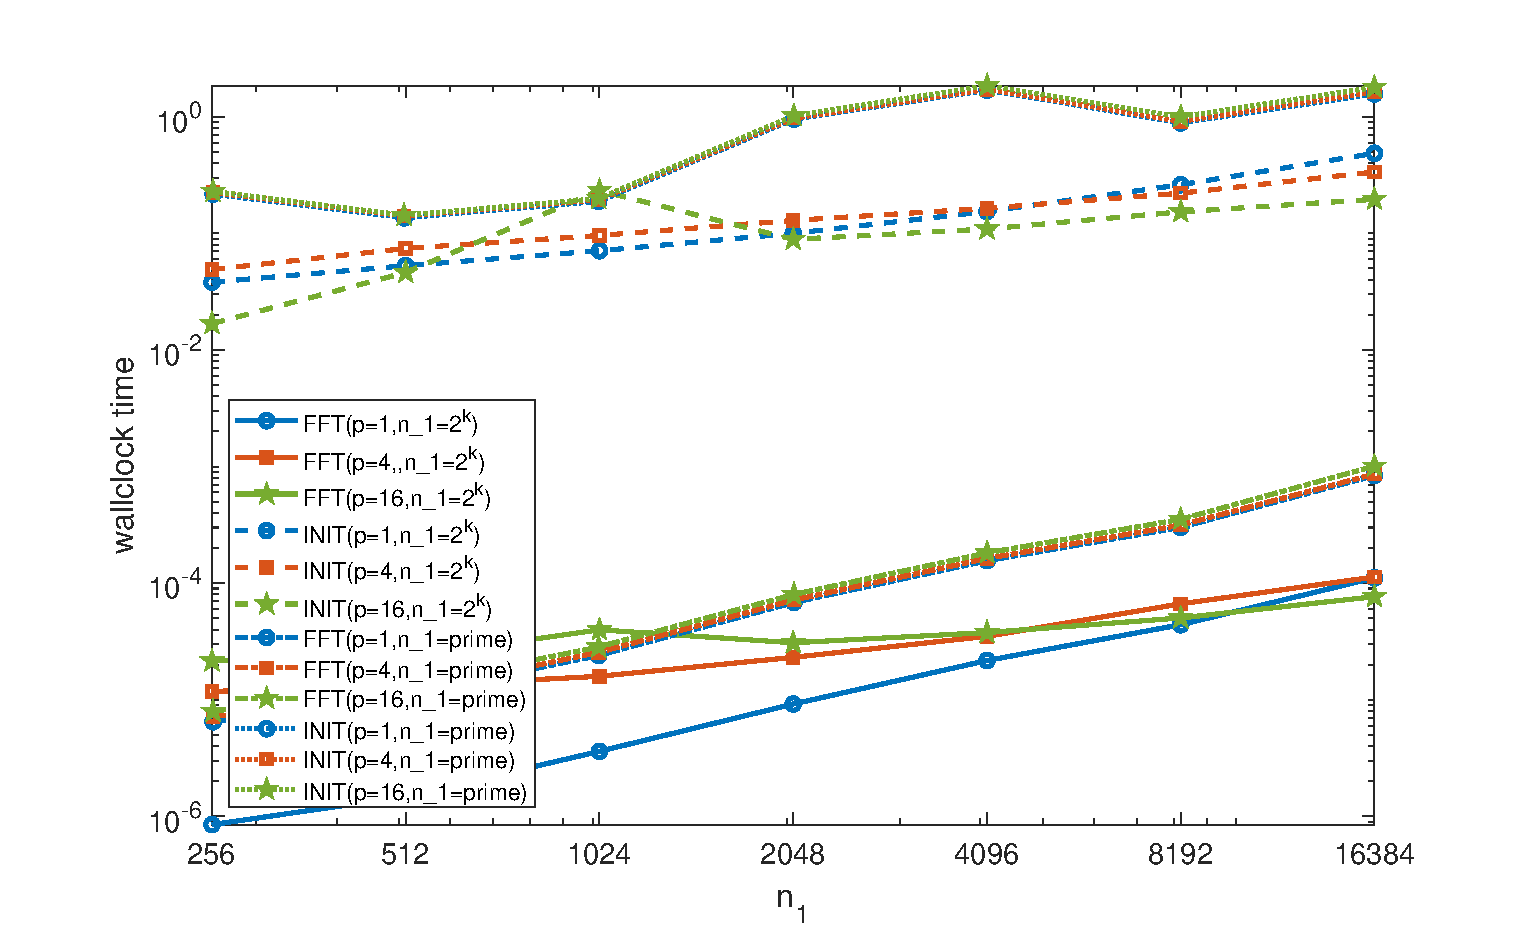
\includegraphics[width=.9\textwidth, height=0.42\textheight]{FFTW1D_times_fig.eps}
\caption{1D FFTW applied to real valued one-dimensional arrays of length $n_1$ using $p$ MPI processes. Wallclock initialisation time, INIT, and wallclock FFT time, FFT, are given in seconds.}
\label{Fig:fftw1d_times}
\end{center}
\end{figure}



In Figure~\ref{Fig:fftw1d_threads_times} we fix the number of MPI processes to one and vary the number of OpenMP threads. As with the tests where the number of threads was fixed at one and the number of MPI threads were varied, the problem sizes considered do not see any benefit from using multiple threads until we reach $n_1=16384$ (16381 in the prime tests). 


\begin{figure}[!htbp]
\begin{center}
 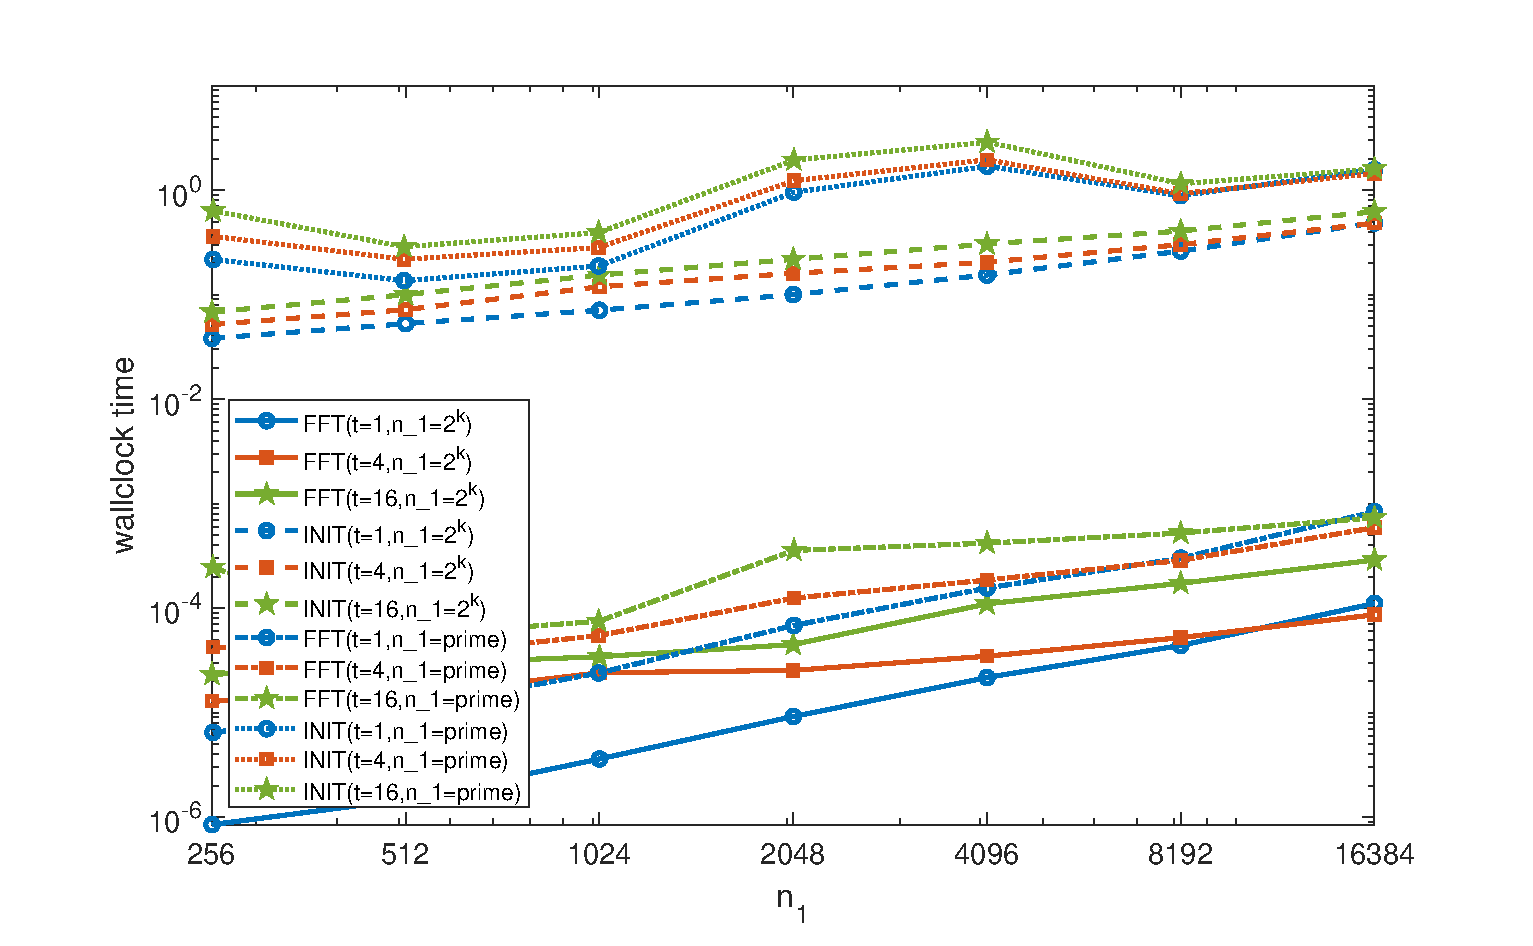
\includegraphics[width=.9\textwidth, height=0.42\textheight]{FFTW1D_threads_times_fig.eps}
\caption{1D FFTW applied to real valued one-dimensional arrays of length $n_1$ using $t$ threads and 1 MPI process. Wallclock initialisation time, INIT, and wallclock FFT time, FFT, are given in seconds.}
\label{Fig:fftw1d_threads_times}
\end{center}
\end{figure}



\begin{figure}[!htbp]
\begin{center}
 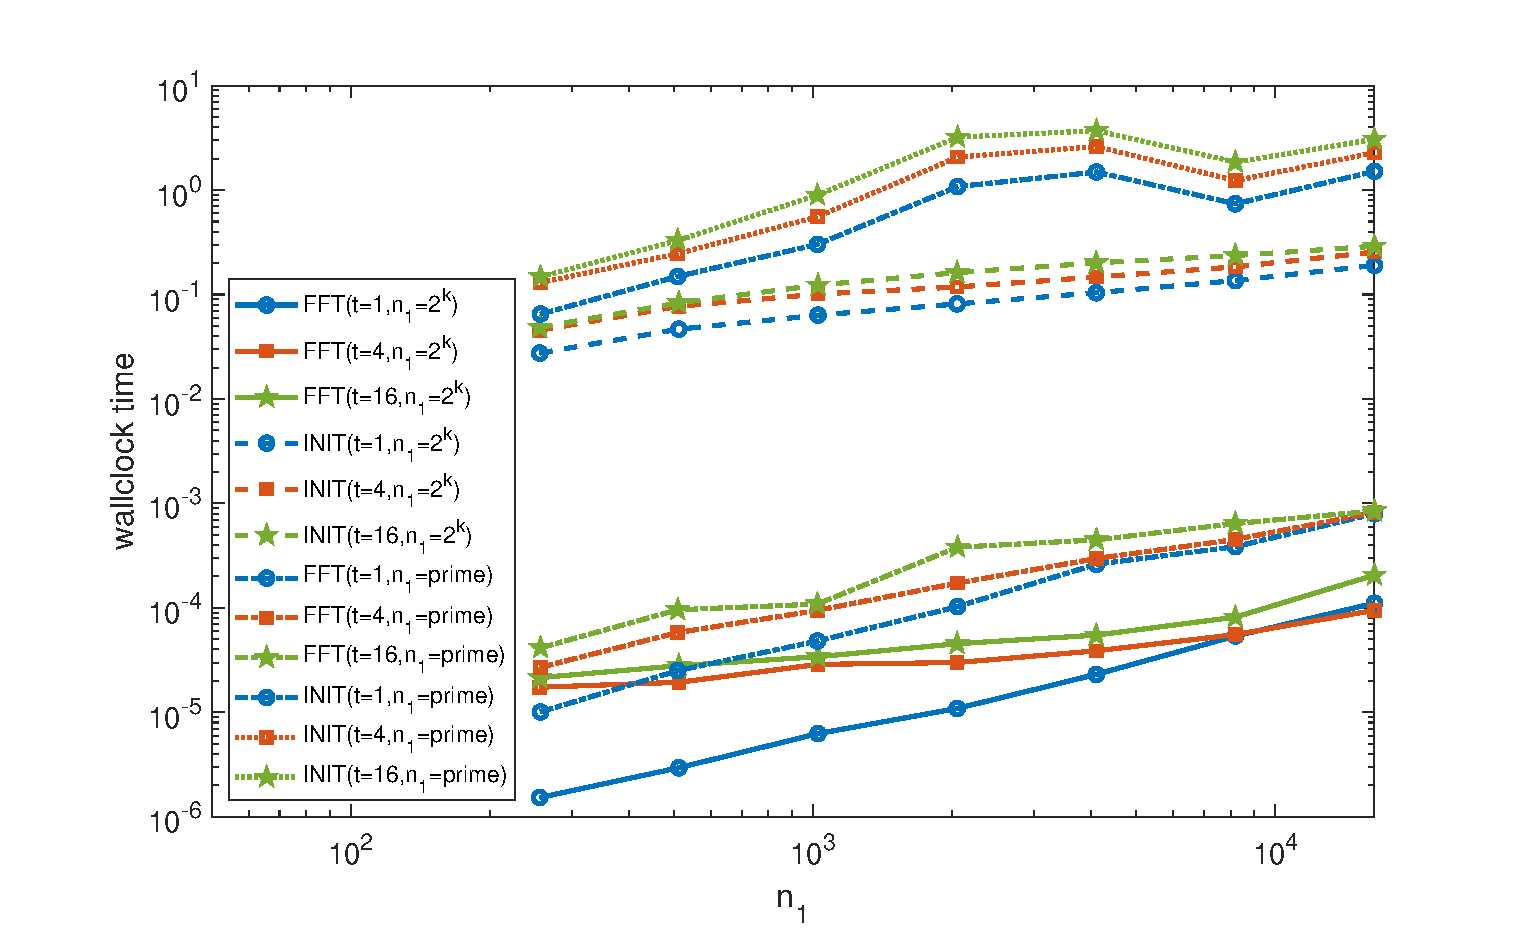
\includegraphics[width=.9\textwidth, height=0.42\textheight]{FFTW1D_OMP_threads_times_fig.eps}
\caption{1D FFTW applied to real valued one-dimensional arrays of length $n_1$ using $t$ threads with the pure OpenMP version. Wallclock initialisation time, INIT, and wallclock FFT time, FFT, are given in seconds.}
\label{Fig:fftw1d_omp_threads_times}
\end{center}
\end{figure}

In Tables~\ref{Tbl:FFT1d2048}, \ref{Tbl:FFT1d2053}, \ref{Tbl:FFT1d16381} and 
\ref{Tbl:FFT1d16384},  the FFT compution and initialisation wallclock times and 
ratios with respect to 1 MPI process combined with 1 OpenMP thread are provided 
for $n_1=2048,$ $n_1=2053,$  $n_1=16381$ and  $n_1=16384,$ respectively. For the 
two smaller problem sizes, fixing the number of MPI processes and increasing the 
number of threads results in a monotonic increase in FFT computation time but the
 rate of increase is, in general, greater for when $n_1$ is a power of 2 than 
when $n_1$ was a prime number. Fixing the number of threads and increasing the 
number of processes results in differeing behaviours between $n_1=2^{11}(=2048)$ 
and $n_1=2053.$ In the latter case, increasing the number of processes generally 
results in a very mild increase in the FFT computation time' the initialisation 
time remains simlar. The optimal initialisation times and FFT computation times 
all occured when there was one MPI process with one OpenMP thread.  When 
$n_1=2^{11},$ increasing the number of processes from one to two but fixing the 
number of threads reults in a large increase in FFT computation time but a milder 
increase in the initialisation time. Increasing the number of MPI processes 
further reduces the initialisation time from when two processes were used and in 
the case of one thread, there is an 11\% reduction time in initialisation time 
when using 16 processes compared to just one process. However, the FFT 
computation time remains significantly higher than when one MPI process was used. 
For $n_1=2^{11},$ the lowest FFT computation time occrred with a single MPI 
processes combined with a single OpenMP thread; the lowest initialisation time 
was when there were 16 MPI processes with a single thread on each process. Thus, 
when running a code that performs multiple FFT computations with $n_1=2^{11},$ it 
is best to use 16 MPI processes with a single thread on each when fewer than 524 
FFT computations are requires; when at least 524 computations are needed, a single 
MPI process with a single thread is optimal in turns of total FFT initialisation 
and computation time. 

 
In Table~\ref{Tbl:FFT1d16381}, $n_1$ is prime; however, $n_1$ is a power of 2 
in Table~\ref{Tbl:FFT1d16384}. Direct comparison of the tables demonstrates the 
optimization of FFTW, with respect to FFT computation time, for values of $n_1$ 
that are products of small integers. For both values of $n_1,$ using a single 
MPI process and increasing the number of threads from 1 until there are eight 
threads results in monotonic decreases in the FFT computation time. However, 
increasing beyond this number of threads was detrimentatl to the FFT computation 
time, particularly when $n_1=16384.$ Conversely, if the number of threads is 
fixed at one, there are only gains in the FFT computation time for 8 or more 
processes compared to using a single MPI process; the initialisation time is 
reduced by 31\% if 4 MPI processes are requested and a 60\% reduction is 
obtained when 16 MPI processes are used. Across all of our runs for $n_1=16381,$ 
the optimal combination was a single MPI process with 4 threads, giving a 30% 
reduction in FFT computation time and a 8\% reduction in initialisation time. 
For $n_1=2^{14},$ the optimal combination is 16 MPI processes with a single thread. 
Again, we emphasis that the Fortran interface for FFTW combined with the ARCHER 
set-up has not allowed us to reach problem sizes where the true advantages from 
the parallel capability of FFTW are reached.



\begin{table}
\begin{center}
%\being{small}
\begin{tabular}{|r|r|r|r|r|r|r|r|r|}
\hline 
     &  & \multicolumn{7}{c|}{$t$} \\ \hline
    $p$  &  & 1           & 2    & 4    & 8    & 12   & 16    & 24  \\ \hline\hline
    -  & ftime &  1.09e-5 &   1.71e-5 &   3.00e-5 &   3.49e-5 &   4.05e-5 &   4.54e-5 &   6.26e-5   \\ 
      & fratio & 1.00 &    1.57 &    2.75 &    3.20 &    3.72 &    4.17 &    5.74   \\ 
     & itime &   8.13e-2 &    1.09e-1 &   1.18e-1 &   1.42e-1 &   1.72e-1 &   1.62e-1 &   2.14e-1    \\ 
     & iratio &    1.00 &    1.34 &    1.45 &    1.75 &    2.12 &    1.99 &    2.63    \\ \hline \hline
    1  & ftime & 9.19e-6 & 2.05e-5 & 2.54e-5 &  2.81e-5 &   4.03e-5 &   4.49e-5 &  1.84e-4 \\ 
      & fratio & 1.0 & 2.23 & 2.76 &  3.06 &   4.39 &  4.89 &  20.0 \\ 
     & itime &  1.00e-1 &   1.18e-1 &   1.60e-1 &   1.96e-1 &   2.53e-1 &   2.18e-1 &   2.79e-1   \\ 
     & iratio &  1.00 &    1.18 &    1.60 &    1.96 &    2.53 &    2.18 &    2.79   \\ \hline
    2  & ftime & 3.05e-5 &  6.39e-5 &  8.63e-5 &  1.08e-4 &  3.95e-4 & - & - \\ 
      & fratio & 3.32 &  6.95 &  9.39 &  11.8 &   43.0 &  &  \\
      & itime &   1.55e-1 &   2.24e-1 &   2.96e-1 &   3.21e-1 &   4.82e-1   &  &  \\
      & iratio &  1.55 &    2.24 &    2.96 &    3.21 &    4.82    &  &  \\ \hline
    4  & ftime &  2.31e-5 &  7.10e-5  & 8.35e-5 & - & - & - & - \\ 
      & fratio & 2.51 &  7.73  & 9.09 &  &  &  &  \\
      & itime &   1.29e-1 &   1.91e-1 &   2.04e-1    &  & & & \\
      & iratio &  1.29 &    1.91 &    2.04    &  & & &  \\ \hline
    8  & ftime & 2.78e-5 &  8.17e-05 & - & - & - & - & - \\ 
      & fratio & 3.03 &  8.89 &  &  &  &  &  \\
      & itime &   1.04e-1 &   1.56e-1    &  & & & & \\
      & iratio & 1.04 &    1.56    &  & & & & \\ \hline
    16 & ftime  & 3.08e-5 & - & - & - & - & - & - \\ 
     & fratio & 3.35 &  &  &  &  &  &  \\
      & itime &   8.87e-2   & & & & & & \\
      & iratio &   0.89  & & & & & & \\ \hline
\end{tabular}
\caption{1D FFTW applied to real valued one-dimensional arrays of length $n_1=2048$ using $p$ MPI processes and $t$ threads, where $p=-$ represents the threaded version of FFTW (non-MPI). The wallclock FFT computation time, ftime, and wallclock FFT initialisation time, itime, both in seconds, are provided. Additionally, for the MPI-OpenMP version of FFTW, the ratio, fratio, of ftime  with ftime($p=1,t=1$) and the ratio, iratio, of itime  with itime($p=1,t=1$) are provided; for the purely threaded version, these ratios are with respect to ftime($p=-,t=1$) and itime($p=-,t=1$.) }\label{Tbl:FFT1d2048}
%\end{small}
\end{center}
\end{table}



\begin{table}
\begin{center}
%\being{small}
\begin{tabular}{|r|r|r|r|r|r|r|r|r|}
\hline 
     &  & \multicolumn{7}{c|}{$t$} \\ \hline
    $p$  &  & 1           & 2    & 4    & 8    & 12   & 16    & 24  \\ \hline\hline
    -  & ftime &  1.03e-4 &   1.20e-4 &   1.73e-4 &   1.93e-4 &   2.50e-4 &   3.81e-4 &   7.14e-4    \\ 
      & fratio &  1.00 &   1.17 &   1.68 &   1.87 &   2.43 &   3.70 &   6.93    \\ 
     & itime &     1.08e0 &   1.71e0 &   2.07e0 &   2.51e0 &   2.93e0 &   3.21e0 &   3.79e0   \\ 
     & iratio &       1.00 &   1.58 &   1.92 &   2.32 &   2.71 &   2.97 &   3.51     \\ \hline \hline
    1  & ftime & 6.84e-5 &  9.10e-5 &  1.25e-4 &  1.66e-4 &  2.91e-4 &  3.57e-4 &  8.80e-4  \\ 
      & fratio & 1.00 &    1.33 &    1.83 &    2.43 &    4.25 &    5.22 &    12.9 \\
     & itime & 9.55e-1 &   9.95e-1 &   1.23e0 &   1.47e0 &   1.79e0 &   1.94e0 &   2.33e0 \\ 
     & iratio & 1.00 &   1.04 &   1.29 &   1.54 &   1.87 &   2.03 &   2.44   \\  \hline
    2  & ftime & 6.89e-5 &  9.29e-5 &  1.34e-4 &  1.69e-4 &  5.52e-4  & - & - \\ 
      & fratio &  1.01 &    1.36 &    1.96 &    2.47 &    8.07     &  &  \\
      & itime &  9.67e-1 &   1.03e0 &   1.24e0 &   1.49e0 &   1.80e0  &  &  \\
      & iratio &  1.01 &   1.08 &   1.30 &   1.56 &   1.88  &  &  \\ \hline
    4  & ftime & 7.17e-5 &  9.96e-5 &  1.33e-4  & - & - & - & - \\ 
      & fratio &  1.05 &    1.46 &    1.94    &  &  &  &  \\
      & itime &  9.73e-1 &   1.03e0 &   1.23e0   &  & & & \\
      & iratio & 1.02 &   1.08 &   1.29   &  & & &  \\ \hline
    8  & ftime &7.62e-5 &  1.02e-4  & - & - & - & - & - \\ 
      & fratio & 1.11 &    1.49    &  &  &  &  &  \\
      & itime &  1.00e0 &   1.04e0  &  & & & & \\
      & iratio &  1.05 &   1.09   &  & & & & \\ \hline
    16 & ftime  &    8.00e-5  & - & - & - & - & - & - \\ 
     & fratio &     1.17   &  &  &  &  &  &  \\
      & itime & 1.02e0   & & & & & & \\
      & iratio & 1.07  & & & & & & \\ \hline
\end{tabular}
\caption{1D FFTW applied to real valued one-dimensional arrays of length $n_1=2053$ using $p$ MPI processes and $t$ threads, where $p=-$ represents the threaded version of FFTW (non-MPI). The wallclock FFT computation time, ftime, and wallclock FFT initialisation time, itime, both in seconds, are provided. Additionally, for the MPI-OpenMP version of FFTW, the ratio, fratio, of ftime  with ftime($p=1,t=1$) and the ratio, iratio, of itime  with itime($p=1,t=1$) are provided; for the purely threaded version, these ratios are with respect to ftime($p=-,t=1$) and itime($p=-,t=1$.) }\label{Tbl:FFT1d2053}
%\end{small}
\end{center}
\end{table}


\begin{table}
\begin{center}
%\being{small}
\begin{tabular}{|r|r|r|r|r|r|r|r|r|}
\hline 
     &  & \multicolumn{7}{c|}{$t$} \\ \hline
    $p$  &  & 1           & 2    & 4    & 8    & 12   & 16    & 24  \\ \hline\hline
    -  & ftime &  7.97e-4 &   7.98e-4 &   8.19e-4 &   8.25e-4 &   8.30e-4 &   8.47e-4 &   9.57e-4     \\ 
      & fratio &   1.00 &   1.00 &   1.03 &   1.04 &   1.04 &   1.06 &   1.20    \\ 
     & itime &   1.51e0 &   2.05e0 &   2.29e0 &   2.56e0 &   2.84e0 &   3.07e0 &   3.67e0     \\ 
     & iratio &   1.00 &   1.36 &   1.52 &   1.70 &   1.88 &   2.03 &   2.43     \\ \hline \hline
    1  & ftime &  8.38e-4 &  6.01e-4 &  5.90e-4 &  5.89e-4 &  7.43e-4 &  7.33e-4 &  9.93e-4  \\ 
      & fratio & 1.00 &  0.72 &  0.70 &  0.70 &  0.89 &  0.87 &  1.19   \\ 
     & itime & 1.57e0 &   1.55e0 &   1.45e0 &   1.50e0 &   1.59e0 &   1.60e0 &   1.84e0  \\ 
     & iratio & 1.00 &   0.99 &   0.92 &   0.96 &   1.01 &   1.02 &   1.17  \\ \hline
    2  & ftime &  7.96e-4 &  6.49e-4 &  6.32e-4 &  6.08e-4 &  8.62e-4  & - & - \\ 
      & fratio &   0.95 &  0.77 &  0.75 &  0.73 &  1.03   &  &  \\
      & itime &  1.59e0 &   1.57e0 &   1.48e0 &   1.49e0 &   1.64e0   &  &  \\
      & iratio &  1.01 &   1.00 &   0.94 &   0.95 &   1.04  &  &  \\ \hline
    4  & ftime & 8.62e-4 &  6.67e-4 &  6.03e-4   & - & - & - & - \\ 
      & fratio &   1.03 &  0.80 &  0.72  &  &  &  &  \\
      & itime &  1.63e0 &   1.57e0 &   1.51e0   &  & & & \\
      & iratio &  1.03 &   1.00 &   0.96  &  & & &  \\ \hline
    8  & ftime &  8.40e-4 &  6.99e-4    & - & - & - & - & - \\ 
      & fratio & 1.00 &  0.83  &  &  &  &  &  \\
      & itime &  1.71e0 &   1.70e0   &  & & & & \\
      & iratio &  1.09 &   1.08  &  & & & & \\ \hline
    16 & ftime  & 1.01e-3    & - & - & - & - & - & - \\ 
     & fratio &  1.21   &  &  &  &  &  &  \\
      & itime &   1.79e0  & & & & & & \\
      & iratio & 1.14   & & & & & & \\ \hline
\end{tabular}
\caption{1D FFTW applied to real valued one-dimensional arrays of length $n_1=16381$ using $p$ MPI processes and $t$ threads, where $p=-$ represents the threaded version of FFTW (non-MPI). The wallclock FFT computation time, ftime, and wallclock FFT initialisation time, itime, both in seconds, are provided. Additionally, for the MPI-OpenMP version of FFTW, the ratio, fratio, of ftime  with ftime($p=1,t=1$) and the ratio, iratio, of itime  with itime($p=1,t=1$) are provided; for the purely threaded version, these ratios are with respect to ftime($p=-,t=1$) and itime($p=-,t=1$.) }\label{Tbl:FFT1d16381}
%\end{small}
\end{center}
\end{table}

\begin{table}
\begin{center}
%\being{small}
\begin{tabular}{|r|r|r|r|r|r|r|r|r|}
\hline 
     &  & \multicolumn{7}{c|}{$t$} \\ \hline
    $p$  &  & 1           & 2    & 4    & 8    & 12   & 16    & 24  \\ \hline\hline
    -  & ftime & 1.11e-4 &   8.58e-5 &   9.49e-5 &   8.59e-5 &   9.79e-5 &   2.06e-4 &   5.42e-4   \\ 
      & fratio & 1.00 &   0.77 &   0.85 &   0.77 &   0.88 &   1.86 &   4.88  \\
     & itime &  1.90e-1 &   2.62e-1 &   2.55e-1 &   2.60e-1 &   3.07e-1 &   2.90e-1 &   3.98e-1   \\ 
     & iratio &  1.00 &   1.38 &   1.34 &   1.37 &   1.62 &   1.53 &   2.09   \\  \hline \hline
    1  & ftime &   1.11e-4 &  9.20e-5 &  8.65e-5 &  7.81e-5 &  3.35e-4&   2.89e-4 &  5.16e-4  \\ 
      & fratio & 1.0000 &   0.83 &   0.78 &   0.70 &   3.02 &   2.60 &   4.65   \\
     & itime & 4.86e-1 &   4.82e-1 &   4.84e-1 &   5.41e-1 &   6.23e-1 &   6.21e-1 &   7.27e-1  \\ 
     & iratio &  1.00 &   0.99 &  1.00 &   1.11 &   1.28 &   1.28 &   1.50  \\  \hline
    2  & ftime & 1.93e-4  & 2.51e-4 &  2.88e-4 &  3.27e-4 &  8.46e-4  & - & - \\ 
      & fratio &   1.74 &   2.26 &   2.59 &   2.95 &   7.62    &  &  \\
      & itime &     5.10e-1 &   6.58e-1 &   9.09e-1 &   1.02e0 &   1.43e0   &  &  \\
      & iratio & 1.05 &   1.35 &   1.87 &   2.10 &   2.94   &  &  \\ \hline
    4  & ftime &  1.13e-4 &  1.94e-4 &  3.46e-4 & - & - & - & - \\ 
      & fratio &   1.02 &   1.75 &   3.12   &  &  &  &  \\ 
      & itime &   3.36e-1 &   4.64e-1 &   5.18e-1  &  & & & \\
      & iratio & 0.69 &   0.95 &   1.07   &  & & &  \\\hline
    8  & ftime & 8.44e-5 &  1.66e-4   & - & - & - & - & - \\ 
      & fratio &  0.76 &   1.50   &  &  &  &  &  \\
      & itime &  2.34e-1 &   3.53e-1   &  & & & & \\
      & iratio &  0.48 &   0.73  &  & & & & \\ \hline
    16 & ftime  &  7.66e-5   & - & - & - & - & - & - \\ 
     & fratio &    0.69  &  &  &  &  &  &  \\
      & itime &  1.96e-1   & & & & & & \\
      & iratio & 0.40   & & & & & & \\ \hline
\end{tabular}
\caption{1D FFTW applied to real valued one-dimensional arrays of length $n_1=16384$ using $p$ MPI processes and $t$ threads, where $p=-$ represents the threaded version of FFTW (non-MPI). The wallclock FFT computation time, ftime, and wallclock FFT initialisation time, itime, both in seconds, are provided. Additionally, for the MPI-OpenMP version of FFTW, the ratio, fratio, of ftime  with ftime($p=1,t=1$) and the ratio, iratio, of itime  with itime($p=1,t=1$) are provided; for the purely threaded version, these ratios are with respect to ftime($p=-,t=1$) and itime($p=-,t=1$.) }\label{Tbl:FFT1d16384}
%\end{small}
\end{center}
\end{table}

\subsubsection{Complex value arrays}

The results shown in Section~\ref{Sec:FFTWReal} are for real-valued inputs. For 
the mixed Open-MPI version of the FFTW library, the initialisation and  FFT 
calculation times are very similar for both complex and real inputs. For the pure OpenMP version, the FFT calculation times are also very similar 
when comparing complex and real inputs. However, the initilisation times  for $n_1=16384$ and   the complex value interface are between 1.7 and 1.99 times larger than those of the real value interface when multiple threads are used; if a single thread is used, the initiliasation time is 2.88 times larger than the real interface. 



\subsection{MKL}
Whilst the FFTW library was limited in problem size for 1D real problems, the MKL library with MPI provision only has an interface for complex input.



\begin{figure}[!htbp]
\begin{center}
 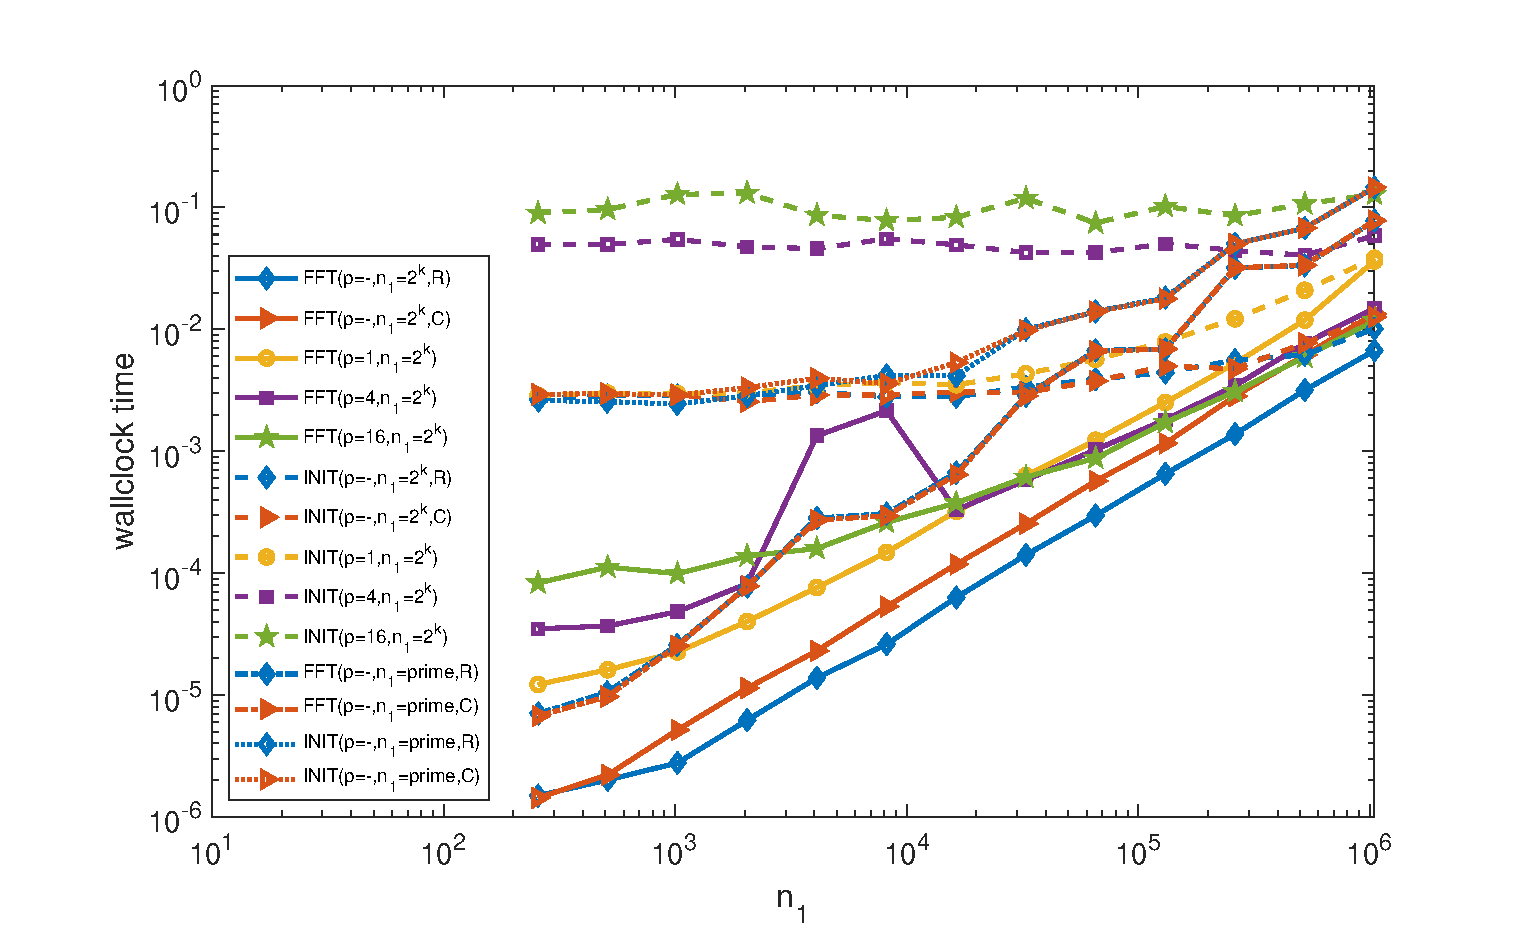
\includegraphics[width=.9\textwidth, height=0.42\textheight]{MKL1D_times_fig.eps}
\caption{1D MKL applied to real valued one-dimensional arrays of length $n_1$ using $p$ MPI processes. Wallclock initialisation time, INIT, and wallclock FFT time, FFT, are given in seconds.}
\label{Fig:mkl1d_times}
\end{center}
\end{figure}




\begin{figure}[!htbp]
\begin{center}
 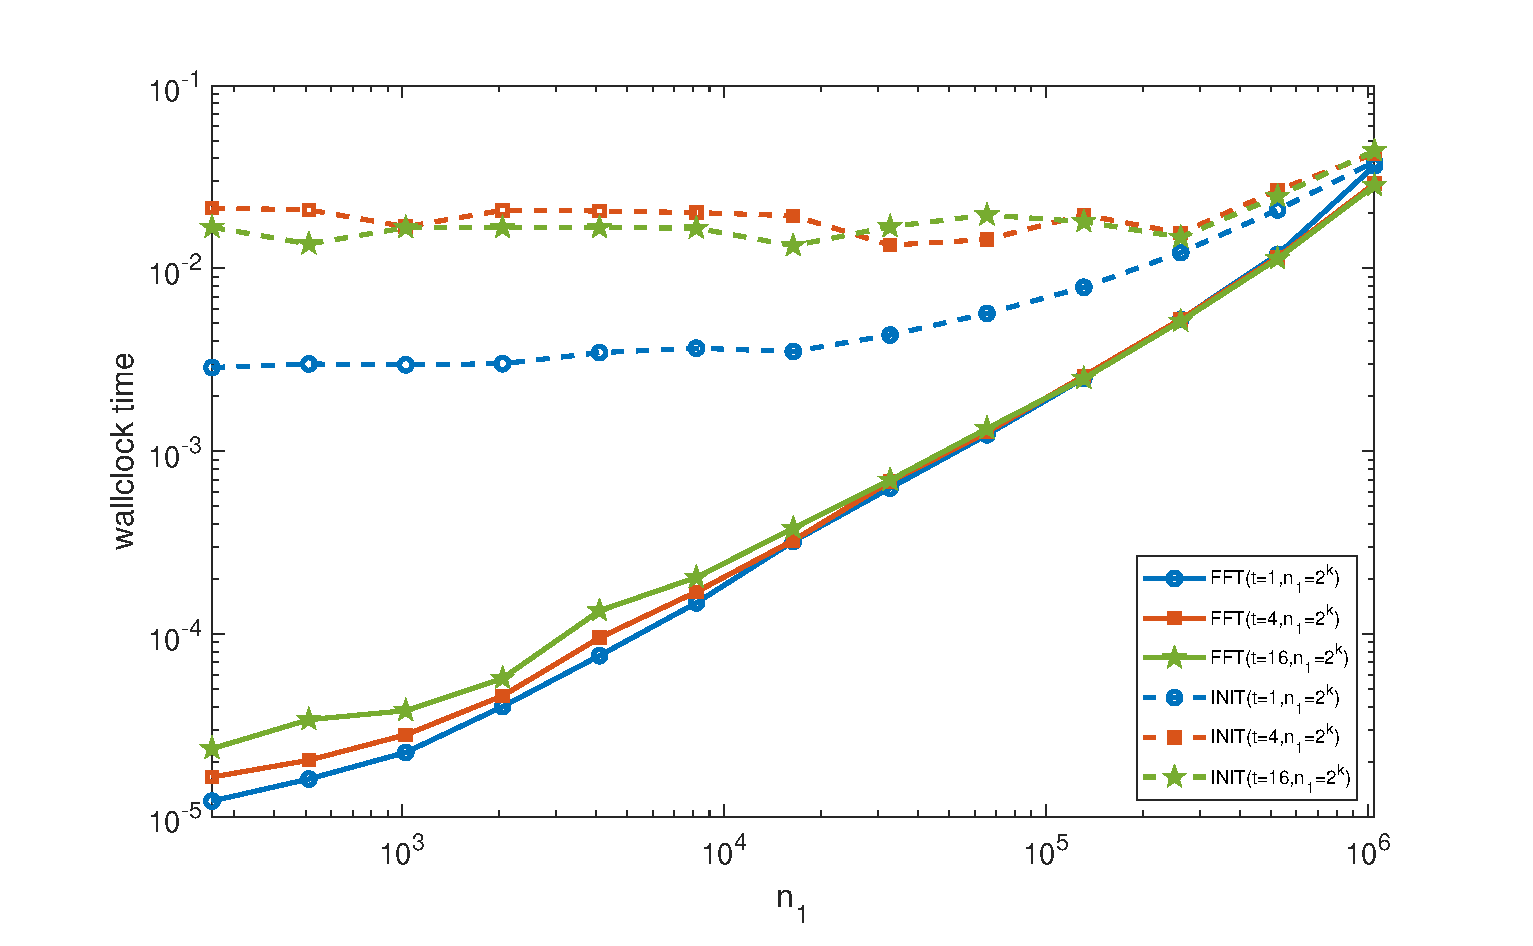
\includegraphics[width=.9\textwidth, height=0.42\textheight]{MKL1D_threads_times_fig.eps}
\caption{1D MKL applied to real valued one-dimensional arrays of length $n_1$ using $t$ threads and 1 MPI process. Wallclock initialisation time, INIT, and wallclock FFT time, FFT, are given in seconds.}
\label{Fig:mkl1d_threads_times}
\end{center}
\end{figure}


\begin{figure}[!htbp]
\begin{center}
 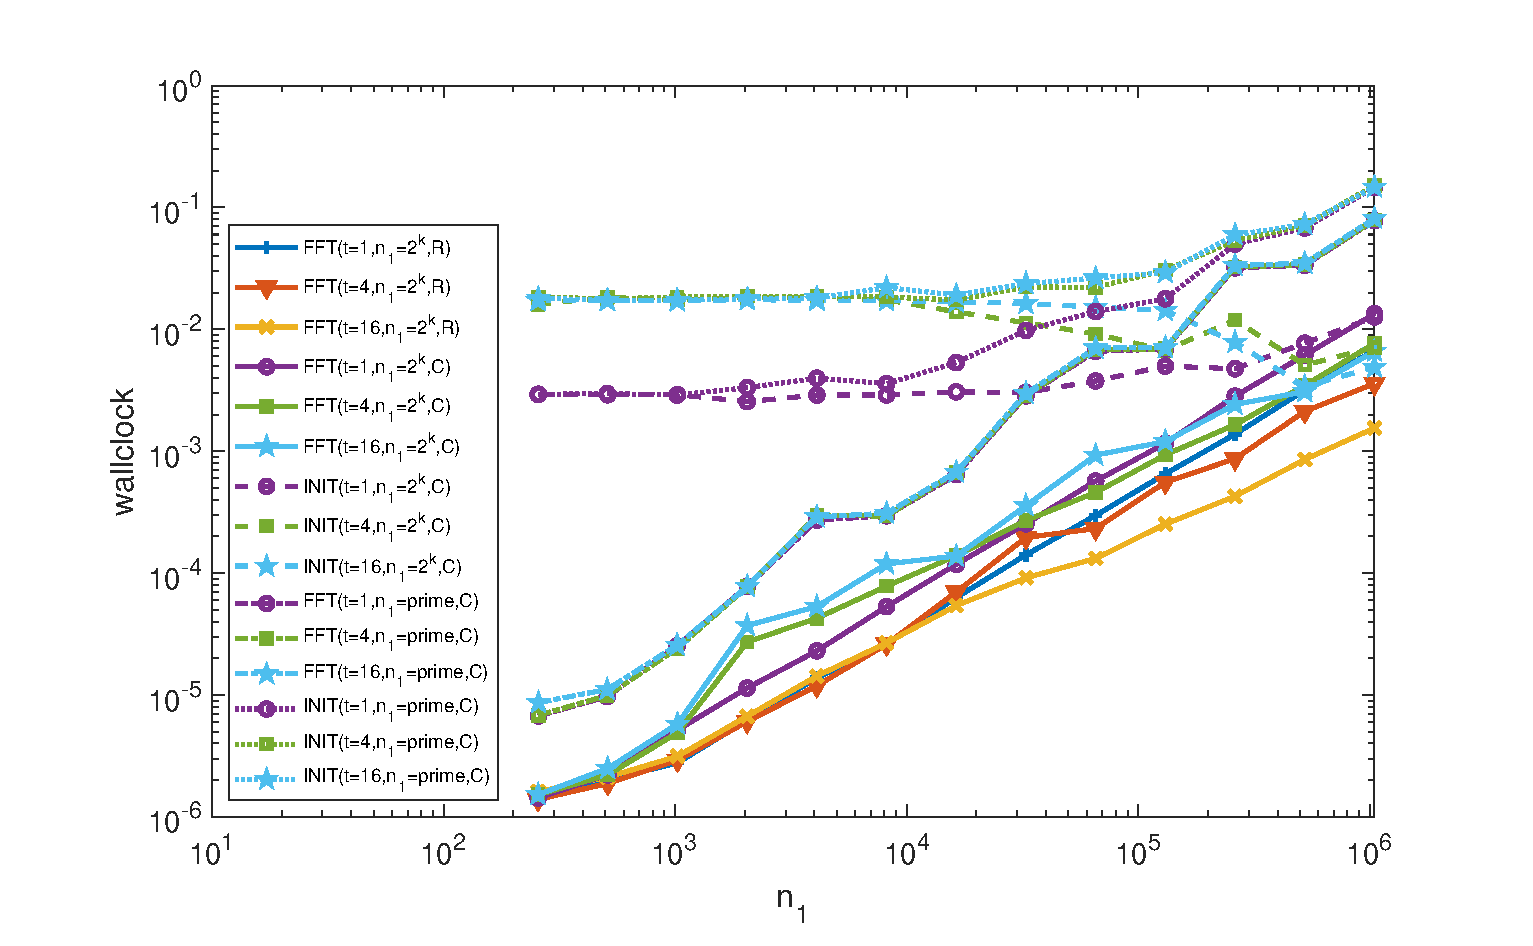
\includegraphics[width=.9\textwidth, height=0.42\textheight]{MKL1D_OMP_threads_times_fig.eps}
\caption{1D MKL (OpenMP version) applied to real valued one-dimensional arrays of length $n_1$ using $t$ threads. Wallclock initialisation time, INIT, and wallclock FFT time, FFT, are given in seconds. The initialisation times for the real and complex interfaces very similar so the times for the real interface are omitted. Additionally, the FFT times are very similar for the real and complex interfaces when $n_1$ is prime and, hence, the times for the real interface are also omitted.}
\label{Fig:mkl1d_omp_threads_times}
\end{center}
\end{figure}



\begin{table}
\begin{center}
%\being{small}
\begin{tabular}{|r|r|r|r|r|r|r|r|r|}
\hline 
     &  & \multicolumn{7}{c|}{$t$} \\ \hline
    $p$  &  & 1           & 2    & 4    & 8    & 12   & 16    & 24  \\ \hline\hline
    -R  & ftime &  6.21e-6 &   8.79e-6 &   6.05e-6 &   6.38e-6 &   7.32e-6 &   6.69e-6 &   7.08e-6    \\ 
      & fratio &   1.00 &   1.42 &   0.97 &   1.03 &   1.18 &   1.08 &   1.14    \\ 
     & itime &      2.82e-3 &   1.27e-2 &   1.83e-2 &   1.72e-2 &   1.75e-2 &   1.67e-2 &   1.66e-2  \\ 
     & iratio &    1.00 &   4.50 &   6.49 &   6.10 &   6.21 &   5.92 &   5.89    \\ \hline
    -C  & ftime &  1.14e-5 &   2.07e-5 &   2.72e-5 &   3.58e-5 &   3.76e-5 &   3.71e-5 &   3.81e-5   \\ 
      & fratio &   1.00 &   1.82 &   2.39 &   3.14 &   3.30 &   3.25 &   3.34  \\ 
     & itime &   2.55e-3 &   1.15e-2 &   1.83e-2 &   2.52e-2 &   1.71e-2 &   1.75e-2 &   1.63e-2    \\ 
     & iratio &    1.00 &   4.51 &   7.18 &   9.88 &   6.71 &   6.86 &   6.39     \\ \hline \hline
    1  & ftime &  4.01e-5 &   4.45e-5 &   4.59e-5 &   5.15e-5 &   6.49e-5 &   5.72e-5 &   7.32e-5    \\ 
      & fratio &  1.00 &   1.11 &   1.14 &   1.28 &   1.62 &   1.43 &   1.83    \\ 
     & itime &     3.01e-3 &   2.87e-3 &   2.08e-2 &   2.11e-2 &   1.77e-2 &   1.67e-2 &   1.64e-2   \\ 
     & iratio & 1.00 &   0.95 &   6.91 &   7.01 &   5.88 &   5.55 &   5.45   \\ \hline
    2  & ftime &   6.52e-5 &   7.34e-5 &   7.70e-5 &   8.15e-5 &   8.16e-5 &    - & - \\ 
      & fratio &      1.63 &   1.83 &   1.92 &   2.03 &   2.03 &    &  \\
      & itime &    1.74e-2 &   2.83e-2 &   3.74e-2 &   2.88e-2 &   3.85e-2    & &  \\
      & iratio &   5.78 &   9.40 &   12.4 &   9.57 &   1.28 &   &  \\ \hline
    4  & ftime &   8.18e-5 &   7.62e-5 &   7.96e-5 &   - & - & - & - \\ 
      & fratio &  2.04 &   1.90 &   1.99 &      &  &  &  \\
      & itime &   4.74e-2 &   6.00e-2 &   6.14e-2    &   & & & \\
      & iratio &   15.7 &   19.9 &   20.4 &    & & &  \\ \hline
    8  & ftime &   8.61e-5 &   9.71e-5 &     - & - & - & - & - \\ 
      & fratio &     2.15 &   2.42 &    &  &  &  &  \\
      & itime &       7.88e-2 &   6.02e-2  &    & & & & \\
      & iratio &     26.2 &   20.0 &    & & & & \\ \hline
    16 & ftime  &    1.38e-4 &    - & - & - & - & - & - \\ 
     & fratio &     3.44 &   &  &  &  &  &  \\
      & itime &     1.31e-1 &  & & & & & \\
      & iratio &      43.5 &    & & & & & \\ \hline
\end{tabular}
\caption{1D MKL applied to one-dimensional arrays of length $n_1=2048$ using $p$ MPI processes and $t$ threads, where $p=-R$ represents the threaded version of MKL (non-MPI) applied to real input values and $p=-C$ represents the threaded version applied to complex values. Note that the MPI-OpenMPI version of MKL only has an interface for complex inputs. The wallclock FFT computation time, ftime, and wallclock FFT initialisation time, itime, both in seconds, are provided. Additionally, for the MPI-OpenMP version of FFTW, the ratio, fratio, of ftime  with ftime($p=1,t=1$) and the ratio, iratio, of itime  with itime($p=1,t=1$) are provided; for the purely threaded version, these ratios are with respect to ftime($t=1$) and itime($t=1$). }\label{Tbl:MKL1d2048}
%\end{small}
\end{center}
\end{table}

\begin{table}
\begin{center}
%\being{small}
\begin{tabular}{|r|r|r|r|r|r|r|r|r|}
\hline 
     &  & \multicolumn{7}{c|}{$t$} \\ \hline
    type  &  & 1           & 2    & 4    & 8    & 12   & 16    & 24  \\ \hline\hline
    R  & ftime &  7.74e-5 &   7.99e-5 &   7.77e-5 &   1.06e-4 &  8.25e-5 &   8.11e-5 &   8.33e-5    \\ 
      & fratio & 1.00 &   1.03 &   1.00 &   1.37 &   1.07 &   1.05 &   1.08     \\ 
     & itime &    2.85e-3 &   1.26e-2 &   2.19e-2 &   2.59e-2 &   1.40e-2 &   1.75e-2 &   1.69e-2     \\ 
     & iratio &   1.00 &   4.42 &   7.68 &   9.09 &   4.91 &   6.14 &   5.93    \\ \hline
    C & ftime &  7.81e-5 &   7.73e-5 &   7.77e-5 &   7.87e-5 &   7.92e-5 &   7.76e-5 &   8.06e-5   \\
      & fratio & 1.0000 &   0.99 &   0.99 &   1.01 &   1.01 &   0.99 &   1.03  \\
      & itime &  3.33e-3 &   1.32e-2 &   1.87e-2 &   2.25e-2 &   2.21e-2 &   1.78e-2 &   1.74e-2  \\
      & iratio & 1.00 &   3.96 &   5.62 &   6.76 &   6.64 &   5.35 &   5.23   \\ \hline
\end{tabular}
\caption{1D MKL applied to one-dimensional arrays of length $n_1=2053$ using the pure OpenMP version with $t$ threads, where type R represents real input and type C represents complex input values. The wallclock FFT computation time, ftime, and wallclock FFT initialisation time, itime, both in seconds, are provided. Additionally, the ratio, fratio, of ftime  with ftime($t=1$) and the ratio, iratio, of itime  with itime($t=1$) are provided. The MPI-OpenMP version of MKL does not have provision prime values of $n_1.$  }\label{Tbl:MKL1d2053}
%\end{small}
\end{center}
\end{table}


\begin{table}
\begin{center}
%\being{small}
\begin{tabular}{|r|r|r|r|r|r|r|r|r|}
\hline 
     &  & \multicolumn{7}{c|}{$t$} \\ \hline
    type  &  & 1           & 2    & 4    & 8    & 12   & 16    & 24  \\ \hline\hline
    R  & ftime &  6.68e-4 &   6.47e-4 &   6.73e-4 &   6.81e-4 &   6.68e-4 &   6.84e-4 &   7.32e-4    \\ 
      & fratio &  1.00 &   0.97 &   1.01 &   1.02 &   1.00 &   1.02 &   1.10    \\ 
     & itime &   4.14e-3 &   1.31e-2 &   1.91e-2 &   2.75e-2 &   1.92e-2 &   1.90e-2 &   2.29e-2      \\ 
     & iratio &   1.00 &   3.16 &   4.61 &   6.64 &   4.64 &   4.59 &   5.53    \\ \hline
   C & ftime &    6.42e-4 &   6.65e-4 &   6.66e-4 &   6.77e-4 &   6.67e-4 &   6.74e-4 &   7.02e-4    \\
     & fratio &  1.00 &   1.04 &   1.04 &   1.05 &   1.04 &   1.05 &   1.09   \\
     & itime &   5.33e-3 &   1.29e-2 &   1.74e-2 &   2.69e-2 &   2.32e-2 &   1.91e-2 &   1.91e-2   \\
     & iratio &  1.00 &   2.42 &   3.26 &   5.05 &   4.35 &   3.58 &   3.58    \\ \hline
\end{tabular}
\caption{1D MKL applied to one-dimensional arrays of length $n_1=16381$ using the pure OpenMP version with $t$ threads, where type R represents real input and type C represents complex input values. The wallclock FFT computation time, ftime, and wallclock FFT initialisation time, itime, both in seconds, are provided. Additionally, the ratio, fratio, of ftime  with ftime($t=1$) and the ratio, iratio, of itime  with itime($t=1$) are provided. The MPI-OpenMP version of MKL does not have provision prime values of $n_1.$  }\label{Tbl:MKL1d16381}
%\end{small}
\end{center}
\end{table}


\begin{table}
\begin{center}
%\being{small}
\begin{tabular}{|r|r|r|r|r|r|r|r|r|}
\hline 
     &  & \multicolumn{7}{c|}{$t$} \\ \hline
    $p$  &  & 1           & 2    & 4    & 8    & 12   & 16    & 24  \\ \hline\hline
    -R  & ftime &   6.30e-5 &   6.74e-5 &   6.98e-5 &   5.49e-5 &   6.03e-5 &   5.41e-5 &   6.23e-5   \\ 
      & fratio &    1.00 &    1.07 &    1.11 &    0.87 &   0.96 &   0.86 &   0.99  \\ 
     & itime &    2.80e-3 &   2.68e-3 &   1.53e-2 &   2.59e-2 &   1.70e-2 &   1.71e-2 &   1.60e-2    \\ 
     & iratio &   1.00 &    0.96 &   5.46 &    9.25 &    6.07 &    6.11 &    5.71      \\ \hline 
    -C  & ftime &  1.18e-4 &   1.82e-4 &   1.39e-4 &   1.32e-4 &   1.39e-4 &   1.38e-4 &   1.44e-4     \\ 
      & fratio &  1.00 &   1.54 &   1.18 &   1.12 &   1.18 &   1.17 &   1.22    \\ 
     & itime &    3.07e-3 &   1.06e-2 &   1.39e-2 &   2.49e-2 &   1.71e-2 &   1.68e-2 &   1.65e-2    \\ 
     & iratio &  1.00 &   3.45 &   4.53 &   8.11 &   5.57 &   5.47 &   5.37       \\ \hline \hline
    1  & ftime & 1.84e-4 &   2.03e-4 &   2.12e-4 &   2.37e-4 &   2.44e-4 &   2.45e-4 &   3.12e-4     \\ 
      & fratio &    1.00 &   1.10 &   1.15 &   1.29 &   1.33 &   1.33 &   1.70   \\ 
     & itime &    3.35e-3 &   1.32e-2 &   1.98e-2 &   1.71e-2 &   1.72e-2 &   1.79e-2 &   1.60e-2    \\ 
     & iratio &  1.00 &   3.94 &   5.91 &   5.10 &   5.13 &   5.34 &   4.78     \\ \hline
    2  & ftime &   2.15e-4 &   2.34e-4 &   2.43e-4 &   2.46e-4 &   2.63e-4 &    - & - \\ 
      & fratio &  1.17 &   1.27 &   1.32 &   1.34 &   1.43 &      &  \\
      & itime &   2.13e-2 &   2.64e-2 &   3.12e-2 &   3.52e-2 &   2.50e-2 &      &  \\
      & iratio &    6.36 &   7.88 &   9.31 &   10.5 &   7.46 &    &  \\ \hline
    4  & ftime &  2.65e-4 &   2.20e-4 &   2.17e-4 &    - & - & - & - \\ 
      & fratio &   1.44 &   1.20 &   1.18 &     &  &  &  \\
      & itime &    4.05e-2 &   5.12e-2 &   4.95e-2 &     & & & \\
      & iratio &     12.1 &   15.3 &   14.8 &   & & &  \\ \hline
    8  & ftime &    2.67e-4 &   2.61e-4 &     - & - & - & - & - \\ 
      & fratio &     1.45 &   1.42 &     &  &  &  &  \\
      & itime &   6.85e-2 &   5.52e-2 &         & & & & \\
      & iratio &    20.4 &   16.5 &       & & & & \\ \hline
    16 & ftime  &     3.06e-4 &    - & - & - & - & - & - \\ 
     & fratio &      1.66 &    &  &  &  &  &  \\
      & itime &      1.10e-1 &   & & & & & \\
      & iratio &    32.8 &     & & & & & \\ \hline
\end{tabular}
\caption{1D MKL applied to one-dimensional arrays of length $n_1=16384$ using $p$ MPI processes and $t$ threads, where $p=-R$ represents the threaded version of MKL (non-MPI) applied to real input values and $p=-C$ represents the threaded version applied to complex values. Note that the MPI-OpenMPI version of MKL only has an interface for complex inputs. The wallclock FFT computation time, ftime, and wallclock FFT initialisation time, itime, both in seconds, are provided. Additionally, for the MPI-OpenMP version of FFTW, the ratio, fratio, of ftime  with ftime($p=1,t=1$) and the ratio, iratio, of itime  with itime($p=1,t=1$) are provided; for the purely threaded version, these ratios are with respect to ftime($t=1$) and itime($t=1$).  }\label{Tbl:MKL1d16384}
%\end{small}
\end{center}
\end{table}



\begin{table}
\begin{center}
%\being{small}
\begin{tabular}{|r|r|r|r|r|r|r|r|r|}
\hline 
     &  & \multicolumn{7}{c|}{$t$} \\ \hline
    type  &  & 1           & 2    & 4    & 8    & 12   & 16    & 24  \\ \hline\hline
    R  & ftime &  7.78e-2 &   7.74e-2 &   7.84e-2 &   7.97e-2 &   8.04e-2 &   8.03e-2 &   8.02e-2    \\ 
      & fratio &  1.00 &   0.99 &   1.01 &   1.02 &   1.03 &   1.03 &   1.03    \\ 
     & itime &    1.46e-1 &   1.48e-1 &   1.54e-1 &   1.57e-1 &   1.49e-1 &   1.51e-1 &   1.58e-1     \\ 
     & iratio &   1.00 &   1.01 &   1.05 &   1.08 &   1.02 &   1.03 &   1.08    \\ \hline
    C  & ftime &   7.80e-2 &   7.78e-2 &   7.88e-2 &   8.01e-2 &   8.06e-2 &   8.13e-2 &   8.25e-2   \\ 
      & fratio &  1.00 &   1.00 &   1.01 &   1.03 &   1.03 &   1.04 &   1.06   \\ 
     & itime &    1.46e-1 &   1.49e-1 &   1.52e-1 &   1.60e-1 &   1.50e-1 &   1.47e-1 &   1.59e-1      \\ 
     & iratio &   1.00 &   1.02 &   1.04 &   1.10 &   1.03 &   1.01 &   1.09   \\ \hline
\end{tabular}
\caption{1D MKL applied to one-dimensional arrays of length $n_1=1048573$ using the pure OpenMP version with $t$ threads, where type R represents real input and type C represents complex input values. The wallclock FFT computation time, ftime, and wallclock FFT initialisation time, itime, both in seconds, are provided. Additionally, the ratio, fratio, of ftime  with ftime($t=1$) and the ratio, iratio, of itime  with itime($t=1$) are provided. The MPI-OpenMP version of MKL does not have provision prime values of $n_1.$   }\label{Tbl:MKL1d1048573}
%\end{small}
\end{center}
\end{table}

\begin{table}
\begin{center}
%\being{small}
\begin{tabular}{|r|r|r|r|r|r|r|r|r|}
\hline 
     &  & \multicolumn{7}{c|}{$t$} \\ \hline
    $p$  &  & 1           & 2    & 4    & 8    & 12   & 16    & 24  \\ \hline\hline
    -R  & ftime &  6.71e-3 &   6.21e-3 &   3.59e-3 &   2.17e-3 &   2.31e-3 &   1.55e-3 &   1.78e-3    \\ 
      & fratio &  1.0000 &    0.93 &   0.54 &   0.32 &   0.34 &   0.23 &   0.27   \\ 
     & itime &    1.01e-2 &   1.79e-2 &   1.11e-2 &   1.20e-2 &   6.88e-3 &   1.53e-2 &   1.81e-2    \\ 
     & iratio &   1.0000 &    1.77 &    1.10 &    1.19 &    0.68 &   1.51 &    1.79    \\  \hline
    -C  & ftime &  1.34e-2 &   1.39e-2 &   7.67e-3 &   5.58e-3 &   5.41e-3 &   6.61e-3 &   7.84e-3   \\ 
      & fratio & 1.00 &   1.04 &   0.57 &   0.42 &   0.40 &   0.49 &   0.59    \\ 
     & itime &   1.26e-2 &   3.58e-3 &   7.13e-3 &   1.46e-2 &   5.19e-3 &   4.88e-3 &   1.43e-2     \\ 
     & iratio &  1.00 &   0.28 &   0.57 &   1.16 &   0.41 &   0.39 &   1.13   \\ \hline \hline
    1  & ftime & 3.64e-2 &   3.04e-2 &   2.91e-2 &   2.80e-2 &   2.87e-2 &   2.84e-2 &   2.93e-2     \\ 
      & fratio &  1.0000 &   0.84 &   0.80 &   0.77 &   0.79 &   0.78 &   0.80   \\ 
     & itime &  3.83e-2 &   3.88e-2 &   4.24e-2 &   5.09e-2 &   4.47e-2 &   4.40e-2 &   5.22e-2     \\ 
     & iratio & 1.00 &   1.01 &   1.11 &   1.33 &   1.17 &   1.15 &   1.36      \\ \hline
    2  & ftime & 2.09e-2 &   1.86e-2 &   2.06e-2 &   2.04e-2 &   2.12e-2 &    - & - \\ 
      & fratio &  0.57 &   0.51 &   0.57 &   0.56 &   0.58 &      &  \\
      & itime &  3.61e-2 &   3.53e-2 &   3.77e-2 &   3.76e-2 &   3.70e-2 &      &  \\
      & iratio &    0.94 &   0.92 &   0.98 &   0.98 &   0.97 &   &  \\ \hline
    4  & ftime &   1.49e-2 &   1.56e-2 &   1.62e-2 &  - & - & - & - \\ 
      & fratio &   0.41 &   0.43 &   0.45 &    &  &  &  \\
      & itime &    5.87e-2 &   5.15e-2 &   4.71e-2 &   & & & \\
      & iratio &  1.53 &   1.34 &   1.23 &     & & &  \\ \hline
    8  & ftime &   1.29e-2 &   1.36e-2 &    - & - & - & - & - \\ 
      & fratio &    0.35 &   0.37 &    &  &  &  &  \\
      & itime &    9.15e-2 &   8.33e-2 &       & & & & \\
      & iratio &    2.39 &   2.17 &      & & & & \\ \hline
    16 & ftime  &  1.18e-2 &      - & - & - & - & - & - \\ 
     & fratio &    0.32 &    &  &  &  &  &  \\
      & itime &    1.28e-1 &     & & & & & \\
      & iratio &   3.34 &    & & & & & \\ \hline
\end{tabular}
\caption{1D MKL applied to one-dimensional arrays of length $n_1=1048576$ using $p$ MPI processes and $t$ threads, where $p=-R$ represents the threaded version of MKL (non-MPI) applied to real input values and $p=-C$ represents the threaded version applied to complex values. Note that the MPI-OpenMPI version of MKL only has an interface for complex inputs. The wallclock FFT computation time, ftime, and wallclock FFT initialisation time, itime, both in seconds, are provided. Additionally, for the MPI-OpenMP version of FFTW, the ratio, fratio, of ftime  with ftime($p=1,t=1$) and the ratio, iratio, of itime  with itime($p=1,t=1$) are provided; for the purely threaded version, these ratios are with respect to ftime($t=1$) and itime($t=1$). }\label{Tbl:MKL1d1048576}
%\end{small}
\end{center}
\end{table}




%%%%%%%%%%%%%%%%%%%%%%%%%%%%%%%%%%%%%%%%%%%%%%%%%%

\section{2D Results}




\bibliographystyle{siam}
\bibliography{bib2017}


\end{document}
